\chapter{Bayesian Compressive Sensing}
\label{ch:bcs}
In this chapter, we combine the Compressive Sensing framework from Chapter \ref{ch:cs} with the Bayesian framework from Chapter \ref{ch:rvm}.



% In order to reconstruct the image, we use the estimated posterior mean to ``predict'' what a pixel value $y^*$ should be at a location $x^*$ in which information was missing:
% \begin{equation}
% y^* = \bs w^T\bs\psi(x^*)
% \end{equation}

% \begin{figure}
% \center
% 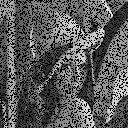
\includegraphics{Images/0.png}
% 
\includegraphics{Images/3.png}
% \caption{Corrupted signal $\bs y$ (left) and reconstructed signal $\hat{\bs x}$ (right) using a cascade of 3 RVMs with Haar basis functions (see \cite{pilikos2014}).}
% \label{fig:lennareconstruction}
% \end{figure}

% Apart from achieving sparse solutions, one further desirable feature of the RVM is that the model provides error bars for its predictions.
% This is used in \cite{pilikos2014} to construct a multi-scale cascade of RVM estimations and achieve significant performance boosts.

% An example of this can be seen in Figure \ref{fig:lennareconstruction}.

